\documentclass{standalone}
\usepackage{tikz}
\usetikzlibrary{patterns, positioning}


\begin{document}
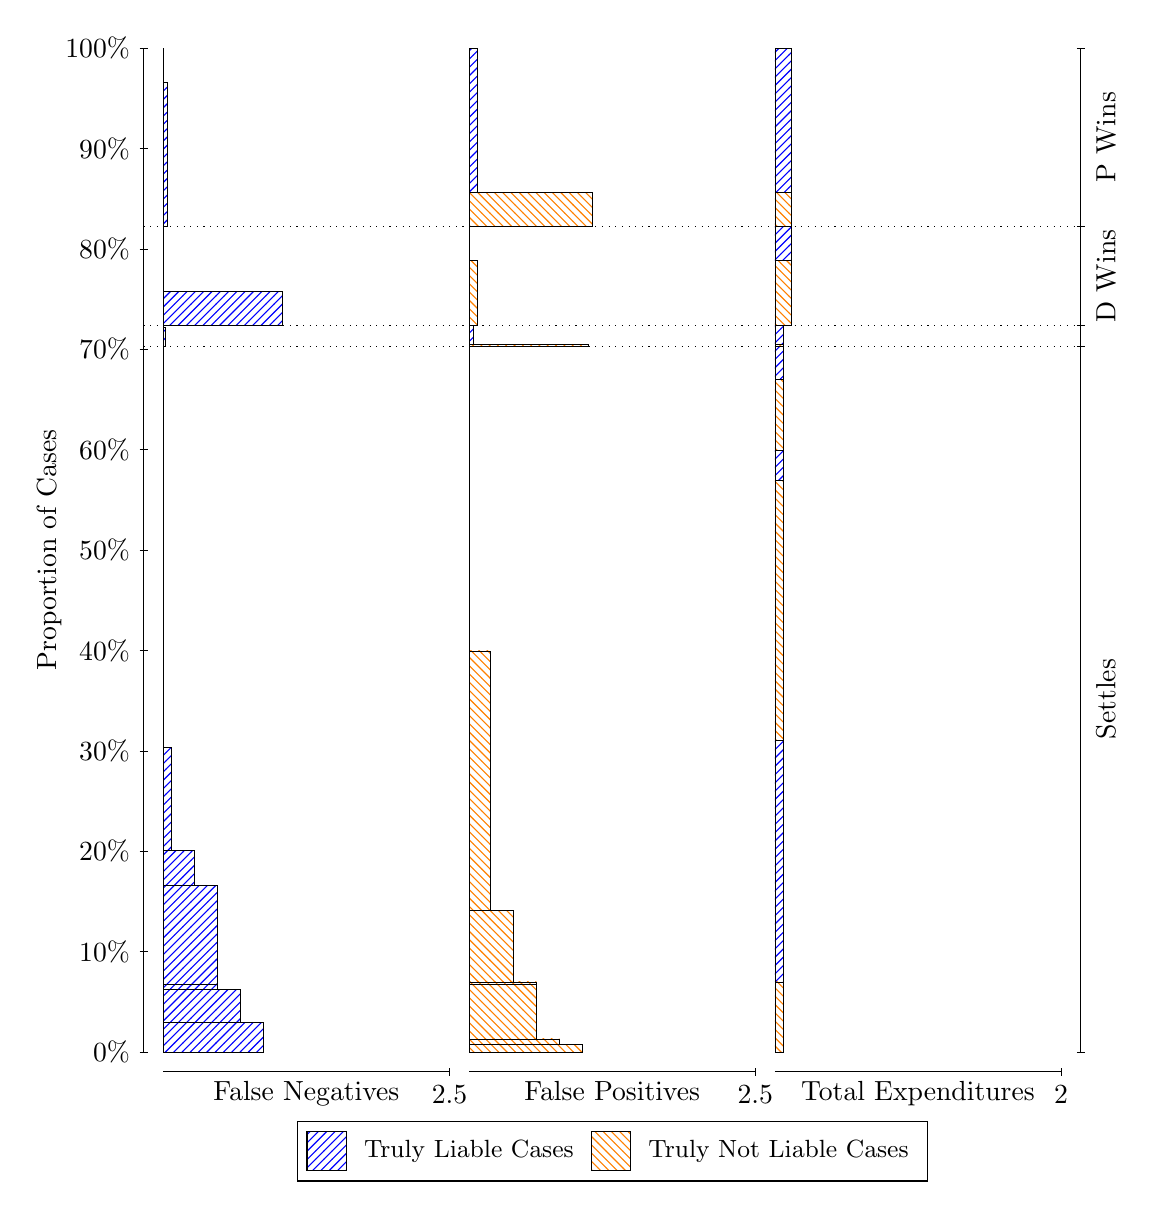
\begin{tikzpicture}
\draw[black, very thin] (1.5,1.75) -- (1.5,14.5);
\node[rotate=90, text=black, anchor=center] at (0.3, 8.125) {Proportion of Cases};
\draw[black, very thin] (1.45,1.75) -- (1.55,1.75);
\node[text=black, anchor=east] at (1.45, 1.75) {0\%};
\draw[black, very thin] (1.45,3.025) -- (1.55,3.025);
\node[text=black, anchor=east] at (1.45, 3.025) {10\%};
\draw[black, very thin] (1.45,4.3) -- (1.55,4.3);
\node[text=black, anchor=east] at (1.45, 4.3) {20\%};
\draw[black, very thin] (1.45,5.575) -- (1.55,5.575);
\node[text=black, anchor=east] at (1.45, 5.575) {30\%};
\draw[black, very thin] (1.45,6.85) -- (1.55,6.85);
\node[text=black, anchor=east] at (1.45, 6.85) {40\%};
\draw[black, very thin] (1.45,8.125) -- (1.55,8.125);
\node[text=black, anchor=east] at (1.45, 8.125) {50\%};
\draw[black, very thin] (1.45,9.4) -- (1.55,9.4);
\node[text=black, anchor=east] at (1.45, 9.4) {60\%};
\draw[black, very thin] (1.45,10.675) -- (1.55,10.675);
\node[text=black, anchor=east] at (1.45, 10.675) {70\%};
\draw[black, very thin] (1.45,11.95) -- (1.55,11.95);
\node[text=black, anchor=east] at (1.45, 11.95) {80\%};
\draw[black, very thin] (1.45,13.225) -- (1.55,13.225);
\node[text=black, anchor=east] at (1.45, 13.225) {90\%};
\draw[black, very thin] (1.45,14.5) -- (1.55,14.5);
\node[text=black, anchor=east] at (1.45, 14.5) {100\%};

\draw[black, very thin] (13.4,1.75) -- (13.4,14.5);
\draw[black, very thin] (13.35,1.75) -- (13.45,1.75);
\node[anchor=west] at (13.35, 1.75) {};
\draw[black, very thin] (13.35,10.715) -- (13.45,10.715);
\node[anchor=west] at (13.35, 10.715) {};
\draw[black, very thin] (13.35,10.975) -- (13.45,10.975);
\node[anchor=west] at (13.35, 10.975) {};
\draw[black, very thin] (13.35,12.234) -- (13.45,12.234);
\node[anchor=west] at (13.35, 12.234) {};
\draw[black, very thin] (13.35,14.5) -- (13.45,14.5);
\node[anchor=west] at (13.35, 14.5) {};

\draw[black, very thin, pattern color=blue, pattern=north east lines] (1.75,1.75) rectangle (3.0126,2.1253);
\draw[black, very thin, pattern color=blue, pattern=north east lines] (1.75,2.1253) rectangle (2.7219,2.5467);
\draw[black, very thin, pattern color=blue, pattern=north east lines] (1.75,2.5467) rectangle (2.4312,2.6054);
\draw[black, very thin, pattern color=blue, pattern=north east lines] (1.75,2.6054) rectangle (2.4312,3.8647);
\draw[black, very thin, pattern color=blue, pattern=north east lines] (1.75,3.8647) rectangle (2.1406,4.3136);
\draw[black, very thin, pattern color=blue, pattern=north east lines] (1.75,4.3136) rectangle (1.8499,5.6198);
\draw[black, very thin, pattern color=orange, pattern=north west lines] (1.75,5.6198) rectangle (1.75,10.715);
\draw[black, very thin, pattern color=blue, pattern=north east lines] (1.75,10.715) rectangle (1.7773,10.955);
\draw[black, very thin, pattern color=orange, pattern=north west lines] (1.75,10.955) rectangle (1.75,10.975);
\draw[black, very thin, pattern color=blue, pattern=north east lines] (1.75,10.975) rectangle (3.2578,11.409);
\draw[black, very thin, pattern color=orange, pattern=north west lines] (1.75,11.409) rectangle (1.75,12.234);
\draw[black, very thin, pattern color=blue, pattern=north east lines] (1.75,12.234) rectangle (1.8045,14.065);
\draw[black, very thin, pattern color=orange, pattern=north west lines] (1.75,14.065) rectangle (1.75,14.5);
\draw[black, very thin, pattern color=orange, pattern=north west lines] (5.6333,1.75) rectangle (7.0685,1.843);
\draw[black, very thin, pattern color=orange, pattern=north west lines] (5.6333,1.843) rectangle (6.7778,1.9162);
\draw[black, very thin, pattern color=orange, pattern=north west lines] (5.6333,1.9162) rectangle (6.4872,2.6098);
\draw[black, very thin, pattern color=orange, pattern=north west lines] (5.6333,2.6098) rectangle (6.4872,2.6389);
\draw[black, very thin, pattern color=orange, pattern=north west lines] (5.6333,2.6389) rectangle (6.1965,3.5464);
\draw[black, very thin, pattern color=orange, pattern=north west lines] (5.6333,3.5464) rectangle (5.9058,6.845);
\draw[black, very thin, pattern color=blue, pattern=north east lines] (5.6333,6.845) rectangle (5.6333,10.715);
\draw[black, very thin, pattern color=orange, pattern=north west lines] (5.6333,10.715) rectangle (7.1412,10.735);
\draw[black, very thin, pattern color=blue, pattern=north east lines] (5.6333,10.735) rectangle (5.6878,10.975);
\draw[black, very thin, pattern color=orange, pattern=north west lines] (5.6333,10.975) rectangle (5.7423,11.8);
\draw[black, very thin, pattern color=blue, pattern=north east lines] (5.6333,11.8) rectangle (5.6333,12.234);
\draw[black, very thin, pattern color=orange, pattern=north west lines] (5.6333,12.234) rectangle (7.1957,12.669);
\draw[black, very thin, pattern color=blue, pattern=north east lines] (5.6333,12.669) rectangle (5.7423,14.5);
\draw[black, very thin, pattern color=orange, pattern=north west lines] (9.5167,1.75) rectangle (9.6189,2.6389);
\draw[black, very thin, pattern color=blue, pattern=north east lines] (9.5167,2.6389) rectangle (9.6189,5.712);
\draw[black, very thin, pattern color=orange, pattern=north west lines] (9.5167,5.712) rectangle (9.6189,9.0106);
\draw[black, very thin, pattern color=blue, pattern=north east lines] (9.5167,9.0106) rectangle (9.6189,9.3859);
\draw[black, very thin, pattern color=orange, pattern=north west lines] (9.5167,9.3859) rectangle (9.6189,10.293);
\draw[black, very thin, pattern color=blue, pattern=north east lines] (9.5167,10.293) rectangle (9.6189,10.715);
\draw[black, very thin, pattern color=orange, pattern=north west lines] (9.5167,10.715) rectangle (9.6189,10.735);
\draw[black, very thin, pattern color=blue, pattern=north east lines] (9.5167,10.735) rectangle (9.6189,10.975);
\draw[black, very thin, pattern color=orange, pattern=north west lines] (9.5167,10.975) rectangle (9.721,11.8);
\draw[black, very thin, pattern color=blue, pattern=north east lines] (9.5167,11.8) rectangle (9.721,12.234);
\draw[black, very thin, pattern color=orange, pattern=north west lines] (9.5167,12.234) rectangle (9.721,12.669);
\draw[black, very thin, pattern color=blue, pattern=north east lines] (9.5167,12.669) rectangle (9.721,14.5);
\draw[black, dotted] (1.5,10.715) -- (13.4,10.715);
\draw[black, dotted] (1.5,10.975) -- (13.4,10.975);
\draw[black, dotted] (1.5,12.234) -- (13.4,12.234);
\draw[black, very thin] (1.75,1.5) -- (5.3833,1.5);
\node[text=black, anchor=north] at (3.5667, 1.5) {False Negatives};
\draw[black, very thin] (5.3833,1.45) -- (5.3833,1.55);
\node[text=black, anchor=north] at (5.3833, 1.45) {2.5};

\draw[black, very thin] (5.6333,1.5) -- (9.2667,1.5);
\node[text=black, anchor=north] at (7.45, 1.5) {False Positives};
\draw[black, very thin] (9.2667,1.45) -- (9.2667,1.55);
\node[text=black, anchor=north] at (9.2667, 1.45) {2.5};

\draw[black, very thin] (9.5167,1.5) -- (13.15,1.5);
\node[text=black, anchor=north] at (11.333, 1.5) {Total Expenditures};
\draw[black, very thin] (13.15,1.45) -- (13.15,1.55);
\node[text=black, anchor=north] at (13.15, 1.45) {2};

\node[text=black, centered, rotate=90] at (13.72, 6.2324) {Settles};

\node[text=black, centered, rotate=90] at (13.72, 11.605) {D Wins};
\node[text=black, centered, rotate=90] at (13.72, 13.367) {P Wins};

\draw (7.449999999999999,1.5) node[draw=none] (baseCoordinate) {};
\begin{scope}[align=center]
        \matrix[scale=0.5, draw=black, below=0.5cm of baseCoordinate, nodes={draw}, column sep=0.1cm]{
            \node[rectangle, draw, minimum width=0.5cm, minimum height=0.5cm, pattern color=blue, pattern=north east lines] {}; &
            \node[draw=none, font=\small, text=black] (B) {Truly Liable Cases}; &
            \node[rectangle, draw, minimum width=0.5cm, minimum height=0.5cm, pattern color=orange, pattern=north west lines] {}; &
            \node[draw=none, font=\small, text=black] (B) {Truly Not Liable Cases}; \\
            };
\end{scope}

\end{tikzpicture}
\end{document}